\section{Evaluation}
\label{sec:evaluation}

\subsection{Experimental Setup}
In order to get the accurate false positive (FP) probability of a given array of elements, we write a C++ program to produce a large set of elements without duplicates, each element has 20 characters.   

 
Our experiments are mainly conducted on a computer with an Intel(R) Core(TM) i7-920 working at 2.67GHz. It has four cores, each with two threads. The DRAM size of our computer is 16GB. It costs about 1 hour to get a 102,400,000(100M) -element traffic file and more than 3 hours to get a 300M-element traffic file, which is larger than 6GB. Both of the files do not contain any duplicate elements. 
Then we use the two traffic files to do several experiments: False Positive (FP) evaluation test, the optimal k test, and performance test.


\subsection{False Positive Probability Test}

\subsubsection{Basic Test}

First, we collect 26 hash functions from several open source websites. Then we use the 100M-traffic file described above to carry out experiments. After inserting the first 5000(n=5000) elements into SBF,  we set k to be the even number from 2 to 16, and get the optimal m according to the formula: $m=\dfrac{k*n}{ln2}$.



\begin{table}[htbp]
\centering\caption{False positive}
\begin{tabular}{c c c c c}
\hline
	&	\# of FP	&	FP of theory	&	FP of simulation	&	error ratio	(\%)\\
\hline
2	&	24814826	&	0.25003480 	&	0.24814830 	&	-0.7545290 	\\
4	&	6263312	&	0.06250841 	&	0.06263312 	&	0.1995030 	\\
6	&	1565056	&	0.01562703 	&	0.01565056 	&	0.1505790 	\\
8	&	392198	&	0.00390674 	&	0.00392198 	&	0.3901310 	\\
10	&	95314	&	0.00097668 	&	0.00095314 	&	-2.4102060 	\\
12	&	24946	&	0.00024417 	&	0.00024946 	&	2.1670100 	\\
14	&	6166	&	0.00006104 	&	0.00006166 	&	1.0125530 	\\
16	&	1528	&	0.00001526 	&	0.00001528 	&	0.1283920 	\\
\hline
\end{tabular}
\label{table:fp:theory:sim}
\end{table}


We query 100,000,000 elements in the SBF we set up before, and the results are shown in Table \ref{table:fp:theory:sim}. It can be observed that as k increases from 2 to 16, the number of FP decreases from 24814826 to 1528 accordingly, as $k$ increases from 2 to 16. We calculate the FP probability of theory using formula \ref{fBloom}. We define the error ratio as (FP\_sim-FP\_theory)/FP\_theory. The observed error ratio is 2.41% at most. In order to minimize the test error, we carry out more experiments below.




\begin{figure*}[htbp]
\begin{minipage}{0.32\linewidth}
  \centerline{\includegraphics[width=6.2cm]{fperrork4}}
  \centerline{(a) k=4}
\end{minipage}
\hfill
\begin{minipage}{0.32\linewidth}
  \centerline{\includegraphics[width=5.8cm]{fperrork5}}
  \centerline{(b) k=5}
\end{minipage}
\hfill
\begin{minipage}{0.32\linewidth}
  \centerline{\includegraphics[width=5.8cm]{fperrork6}}
  \centerline{(c) k=6}
\end{minipage}
\caption{FP probability error ratio vs. \# of queries with different $k$.}
\label{fig:error:ratio}
\end{figure*}


\begin{figure*}[htbp]
\begin{minipage}{0.32\linewidth}
  \centerline{\includegraphics[width=6.2cm]{FPtheorysimk4}}
  \centerline{(a) k=4}
\end{minipage}
\hfill
\begin{minipage}{0.32\linewidth}
  \centerline{\includegraphics[width=5.8cm]{FPtheorysimk5}}
  \centerline{(b) k=5}
\end{minipage}
\hfill
\begin{minipage}{0.32\linewidth}
  \centerline{\includegraphics[width=5.8cm]{FPtheorysimk6}}
  \centerline{(c) k=6}
\end{minipage}
\caption{FP probability error vs. \# of queries with different $k$.}
\label{fig:error:abso}
\end{figure*}




\begin{figure*}[htbp]
\begin{minipage}{0.32\linewidth}
  \centerline{\includegraphics[width=6.2cm]{NotAcck4}}
  \centerline{(a) k=4}
\end{minipage}
\hfill
\begin{minipage}{0.32\linewidth}
  \centerline{\includegraphics[width=5.8cm]{NotAcck5}}
  \centerline{(b) k=5}
\end{minipage}
\hfill
\begin{minipage}{0.32\linewidth}
  \centerline{\includegraphics[width=5.8cm]{NotAcck6}}
  \centerline{(c) k=6}
\end{minipage}
\caption{FP probability error vs. \# of queries with independent queries.}
\label{fig:error:notAcc}
\end{figure*}



\begin{figure*}[htbp]
\begin{minipage}{0.32\linewidth}
  \centerline{\includegraphics[width=6.2cm]{PCQpsk4}}
  \centerline{(a) k=4}
\end{minipage}
\hfill
\begin{minipage}{0.32\linewidth}
  \centerline{\includegraphics[width=5.8cm]{PCQpsk6}}
  \centerline{(b) k=5}
\end{minipage}
\hfill
\begin{minipage}{0.32\linewidth}
  \centerline{\includegraphics[width=5.8cm]{PCQpsk8}}
  \centerline{(c) k=6}
\end{minipage}
\caption{Query speed (Qps) with different traffic.}
\label{fig:PC:QPS}
\end{figure*}





\begin{figure*}[htbp]
\begin{minipage}{0.32\linewidth}
  \centerline{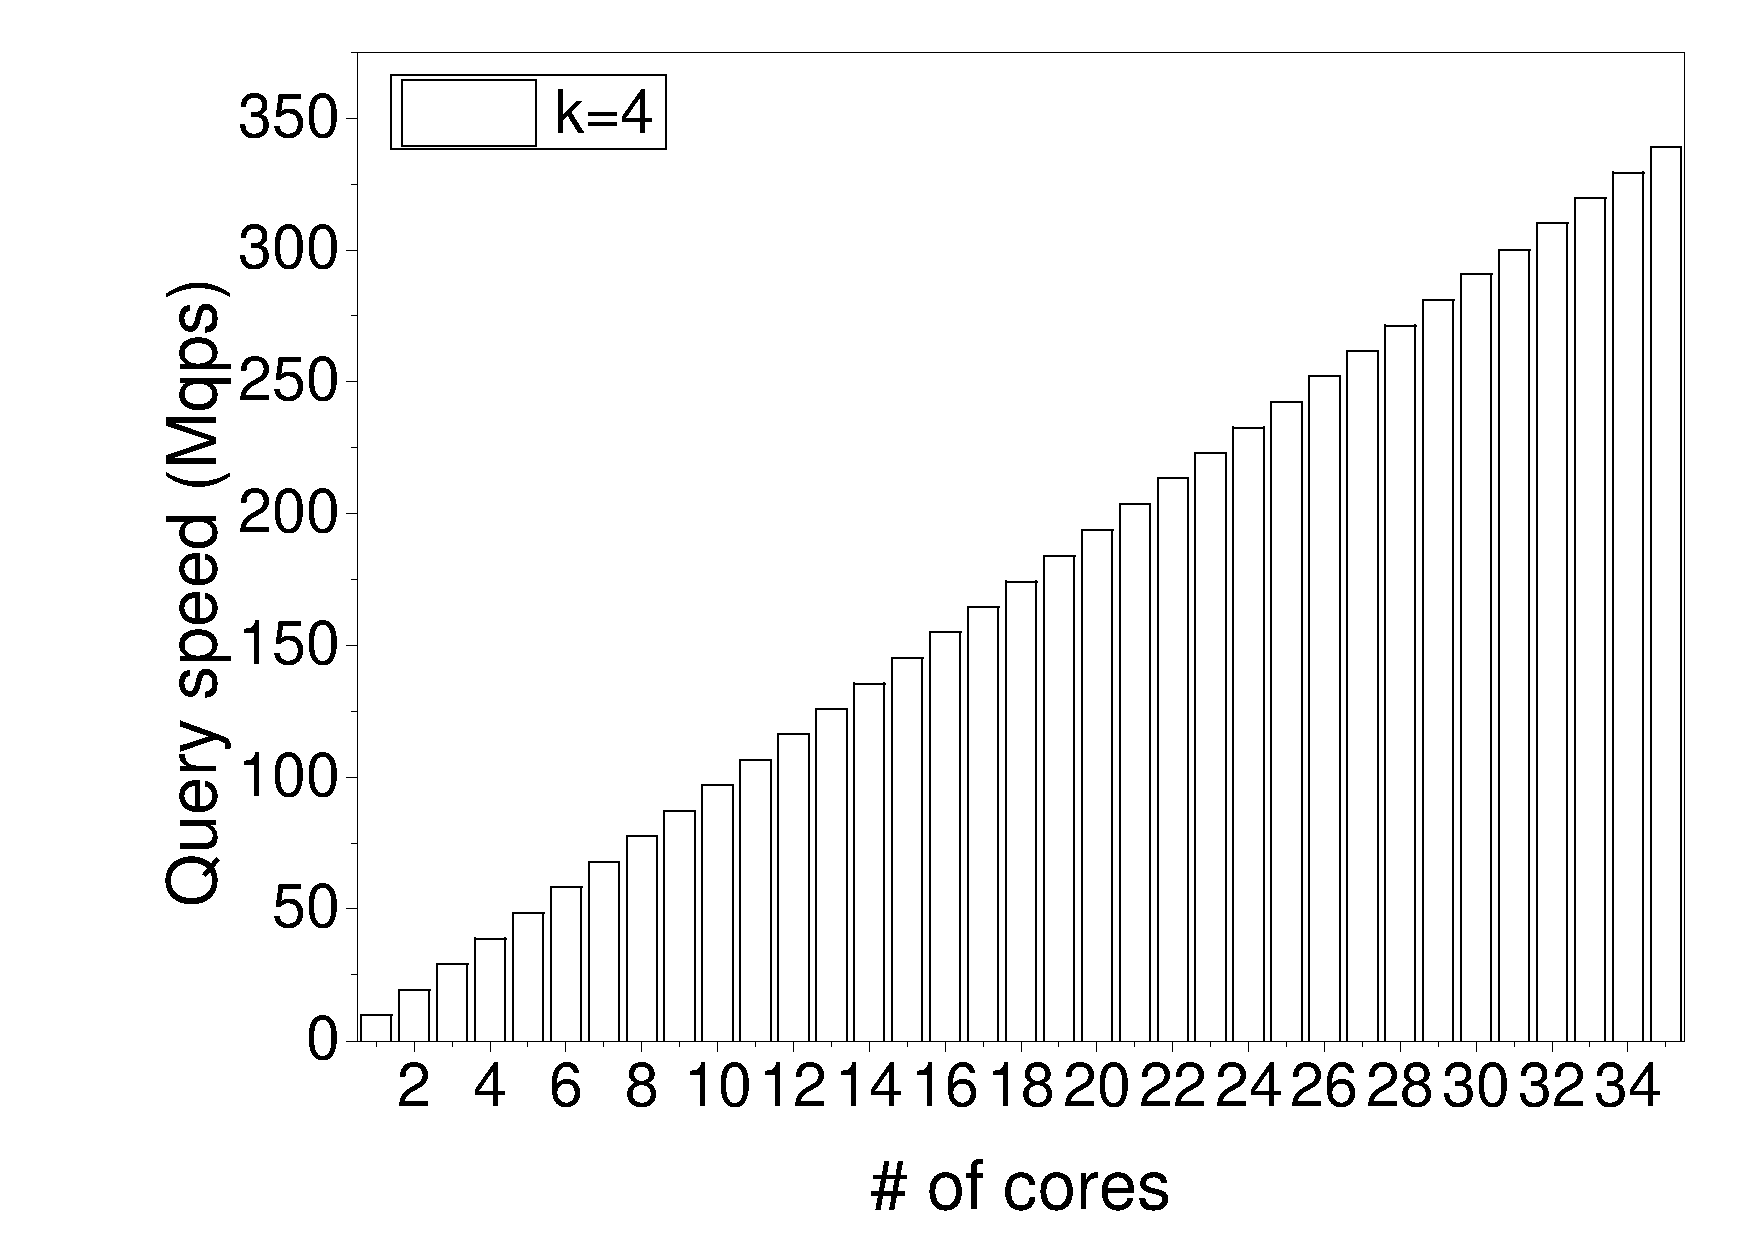
\includegraphics[width=6.2cm]{manyCoreTraffic1}}
  \centerline{(a) Traffic I}
\end{minipage}
\hfill
\begin{minipage}{0.32\linewidth}
  \centerline{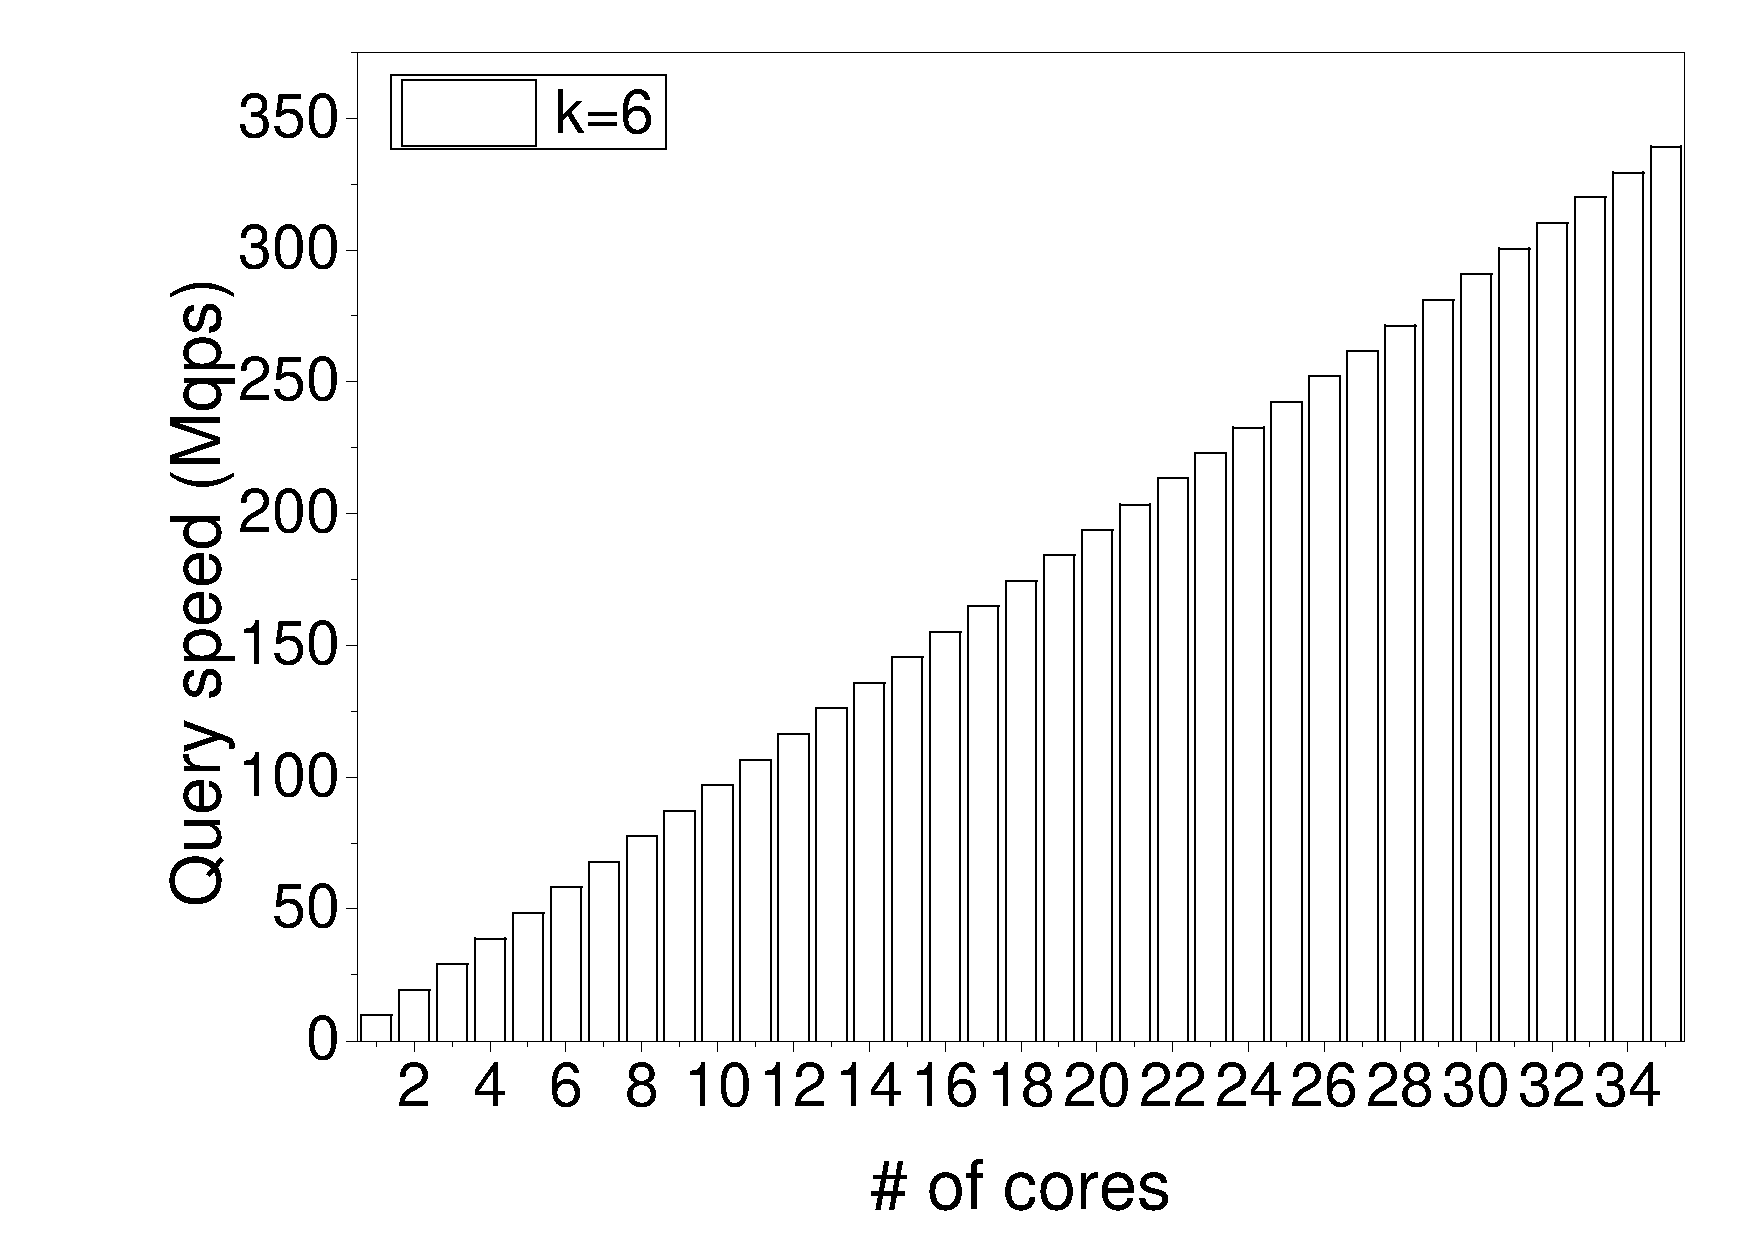
\includegraphics[width=5.8cm]{manyCoreTraffic2}}
  \centerline{(b) Traffic II}
\end{minipage}
\hfill
\begin{minipage}{0.32\linewidth}
  \centerline{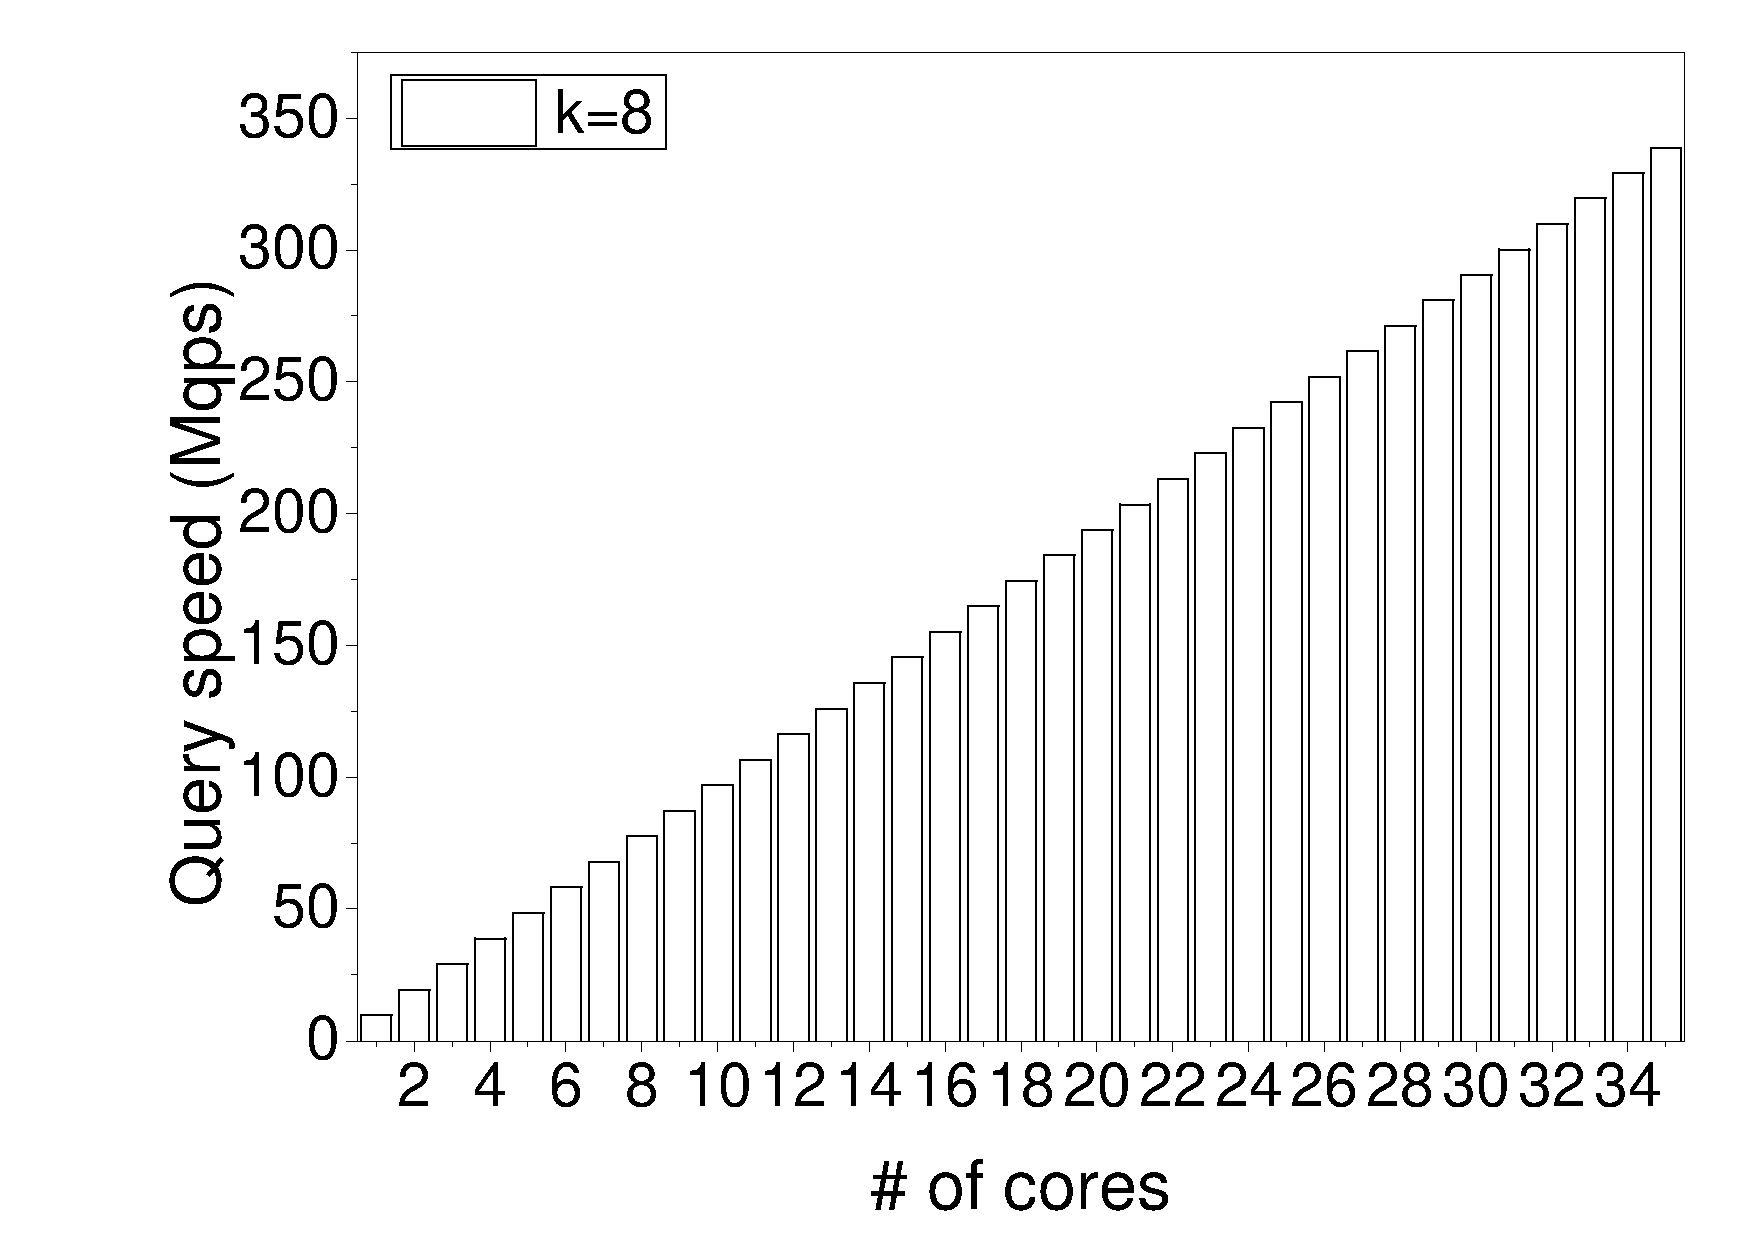
\includegraphics[width=5.8cm]{manyCoreTraffic3}}
  \centerline{(c) Traffic III}
\end{minipage}
\caption{Query speed VS. \# of cores.}
\label{fig:manycore:QPS}
\end{figure*}




